\documentclass[aspectratio=169]{beamer}
\usetheme{madrid}

\usepackage[utf8]{inputenc}
\usepackage[brazil]{babel}

\usepackage{graphicx}


\usebackgroundtemplate%
{%
	
\includegraphics[width=\paperwidth,height=\paperheight]{bg}%
}

\title[MOGESTpy]{Apresentação do MOGESTpy}
\subtitle{Conhecendo o repositório}

\author{Dário Hachisu Hossoda}
\institute[POLI-USP]{Escola Politécnica da Universidade de São Paulo}
\date{\today}

\AtBeginSection[]
{
	\begin{frame}
		\frametitle{Sumário}
		\tableofcontents[currentsection]
	\end{frame}
}

\begin{document}
\frame{\titlepage}

\begin{frame}
	\frametitle{Sumário}
	\tableofcontents
\end{frame}

\section{Os Modelos}

\begin{frame}
\frametitle{O que é o MOGESTpy}
O MOGESTpy é a continuação do projeto desenvolvido durante o estudo de enquadramento da bacia do rio Paranapanema em parceria com a UFPR.

\vspace{1cm}

O nome \alert{MOGESTpy} significa \alert{Mo}delo de \alert{Gest}ão (de Recursos Hídricos) desenvolvido em na linguagem de programação \alert{Py}thon.
\end{frame}

\begin{frame}
\frametitle{Modelo de Gestão em Recursos Hídricos}
Um Modelo de Gestão de Recursos Hídricos contém modelos de qualidade e quantidade que possibilitam a tomada de decisão através da simulação de situações que podem ocorrer na bacia hidrográfica, visto que se trata de um problema de gestão e equações simples de balanço de massa não são satisfatórios para solucionar o problema, por exemplo.
\end{frame}

\begin{frame}
\frametitle{Componentes do MOGESTpy}
O MOGESTpy é composto de modelos de quantidade e qualidade da água em três níveis diferentes:
\begin{block}{Bacia}
SMAP (Soil Moisture Accounting Procedure) + Build Up -- Washoff

Muskingum (routing hidrológico)
\end{block}

\begin{block}{Rio}
SIHQUAL (Equações de Saint-Venant + Equação de advecção -- dispersão -- difusão)
\end{block}

\begin{block}{Reservatório}
Modelo Zero-Dimensional (0D)
\end{block}
\end{frame}

\section{O Repositório}

\begin{frame}
\frametitle{O repositório}
Atualmente o repositório é privado, podendo ser atribuído ao LabSid posteriormente.
\vfill
\begin{block}{Link}
\url{https://github.com/dariohhossoda/MOGESTpy}
\end{block}
\end{frame}

\begin{frame}
\frametitle{Topologia e Organização}
A organização do projeto é feito da seguinte forma:
\vfill
	\begin{itemize}
		\item Quality
		\begin{itemize}
			\item BuWo.py
			\item ZeroD.py
			\item AdvDispDif.py
		\end{itemize}
		\item Quantity
		\begin{itemize}
			\item Hydrological
			\begin{itemize}
				\item SMAP.py
				\item Muskingum.py
			\end{itemize}
			\item Hydrodynamic
			\begin{itemize}
				\item SaintVenant.py
			\end{itemize}
		\end{itemize}
	\end{itemize}
\end{frame}

\begin{frame}
\frametitle{Utilização}
\framesubtitle{Observação Importante}
Por hora, não há uma framework ou interface própria para o modelo. Sendo necessário a utilização dos scripts através de sua utilização a partir de outro arquivo em Python.
\end{frame}

\begin{frame}
\frametitle{Utilização}
\framesubtitle{Ambiente Conda}
Por conta da possibilidade do Python na utilização de diversos pacotes, recomenda-se o ambiente Conda, disponível em: \url{https://conda.io/projects/conda/en/latest/user-guide/install/download.html}

para manter a compatibilidade entre as versões das bibliotecas e do Python em si.

\begin{alertblock}{Miniconda}
A instalação do Miniconda é a mais leve e a indicada.
\end{alertblock}
Confira a documentação nos exemplos do repositório para conseguir utilizar o modelo.
\end{frame}

\begin{frame}
\frametitle{Utilização}
\framesubtitle{Contribuindo com o Projeto}
\begin{columns}
\column{.5\textwidth}
Seguimos o GitFlow (Git Workflow) para a realização de mudanças!
Como fazer sua contribuição?
\vfill
\begin{enumerate}
	\item Crie sua issue (bug/feature);
	\item Crie sua branch linkada ao issue;
	\item Realize um Pull Request ao finalizar.
\end{enumerate}

\column{.5\textwidth}

\begin{figure}[H]
	\centering
	\resizebox{\textwidth}{!}{
		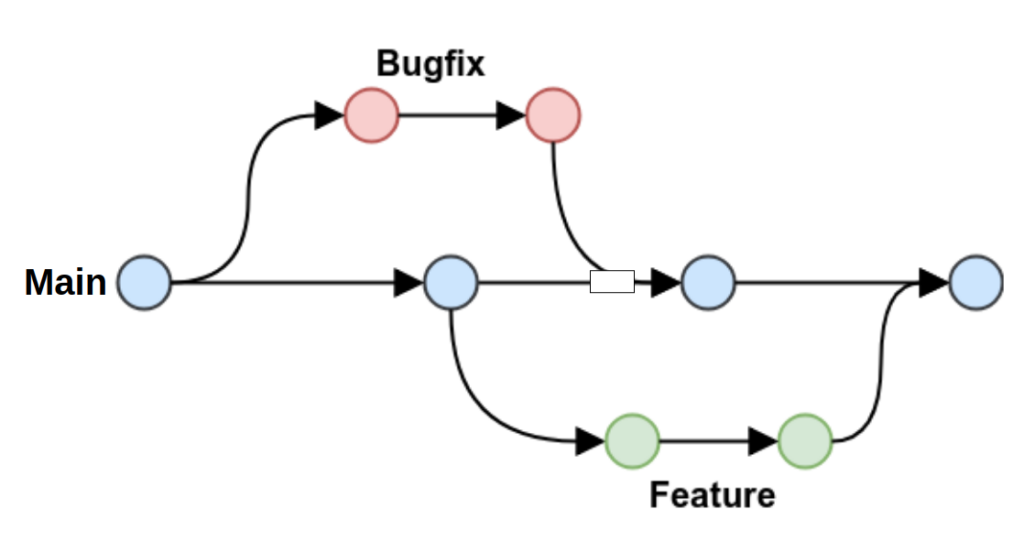
\includegraphics[scale=1.0]{gitflow}
	}
	\caption{Esquema de um projeto que utiliza o GitFlow}
\end{figure}

\end{columns}
\vspace{1cm}
Para mais informações consulte o documento de contribuição.
\end{frame}

\end{document}